% Det offentlige dashbordet: kiindeksen.no

\begin{frame}{kiindeksen.no}
\centering
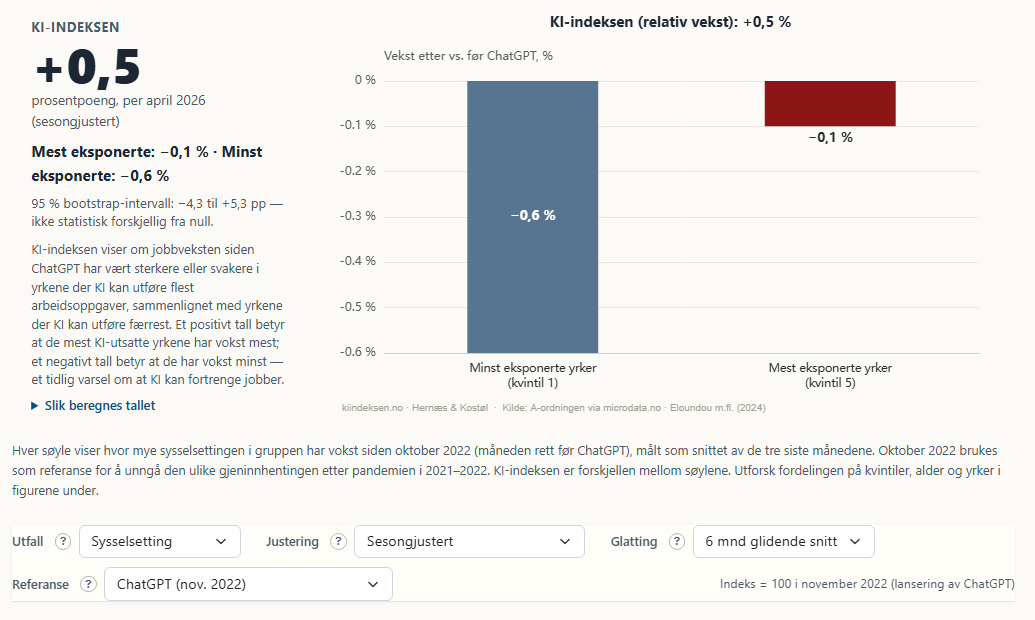
\includegraphics[height=5.9cm,keepaspectratio]{kiindeksen_screenshot.png}

\vspace{0.2em}
\footnotesize
Offentlig dashbord, oppdateres månedlig. Brukeren velger selv utfall, aldersgruppe, enkeltyrker, sesongjustering, glatting og referansemåned. Engelsk versjon på kiindeksen.no/en.
\end{frame}

% ---------------------------------------------------------------
\begin{frame}{Sysselsettingsendring etter kvintil siden ChatGPT}
\centering
\begin{tabular}{lccccc}
\toprule
 & Q1 & Q2 & Q3 & Q4 & Q5 \\
\midrule
Gjennomsnittlig endring (\%) & $-0{,}63$ & $+2{,}94$ & $+0{,}95$ & $+2{,}86$ & $-0{,}09$ \\
\addlinespace
Differanse mot Q1 (\%) & --- & $+3{,}57$ & $+1{,}59$ & $+3{,}49$ & $+0{,}54$ \\
 &  & (5,36) & (2,67) & (2,15) & (2,42) \\
\midrule
Yrker & \multicolumn{5}{c}{374} \\
\bottomrule
\end{tabular}

\vspace{0.8em}
\footnotesize
Endring fra oktober 2022 til snittet av februar--april 2026; sesongjustert antall lønnstakere i privat sektor, 21--60 år, yrker vektet med sysselsettingen i oktober 2022 (som hos Yagan 2019). Mest eksponert $-0{,}09\,\%$ mot minst eksponert $-0{,}63\,\%$: en dobbeltdifferanse på $+0{,}54$ prosentpoeng (SE 2,42), ikke signifikant. Robuste standardfeil over yrker i parentes.
\end{frame}

% ---------------------------------------------------------------
\begin{frame}{kiindeksen.no: en løpende indeks}
\centering

\includegraphics[height=5.2cm,keepaspectratio]{figure_recursive_kiindeks_ci.pdf}

\vspace{0.2em}
\footnotesize
Hovedtallet «KI-indeksen»: sysselsettingsvekst i Q5 mot Q1, siste tre måneder mot oktober 2022. Over voksende datavintager driver tallet fra $+1{,}7$ til $-0{,}2$ og tilbake til $+0{,}5$ prosentpoeng (april 2026). Bootstrap-standardfeil på 2 til 2,5 prosentpoeng hele veien: aldri statistisk skillbar fra null. En reell endring vil vise seg som et varig utslag utenfor båndet.
\end{frame}
